\chapter{Dati}
\label{ch:data}

GroundOne apprende un'unica decisione, e i dati devono insegnare esattamente quella decisione e misurarla in modo
affidabile. Il capitolo definisce dapprima la decisione e le sue etichette, per poi descrivere i tre dataset pubblici
che le forniscono e il modo in cui vengono trasformati in insiemi di addestramento, di sviluppo e di test. Le ultime
sezioni illustrano come l'affidabilità degli insiemi di test sia stata verificata senza nuove annotazioni, che cosa
emerga da un'analisi esplorativa del risultato e come sia stata esclusa la contaminazione tra addestramento e test
(leakage).

% Source of truth for every number in this chapter: Project/data/processed/groundone/DATACARD.md and
% build_report.json (dataset), Project/experiments/eda/report/eda_report.md and stats/ (exploratory analysis).

\section{Compito ed etichette}
\label{sec:data-task}

L'ingresso è costituito da un documento recuperato e da una risposta scritta da un modello linguistico, suddivisa in
frasi. Per ciascuna frase il modello stabilisce se, \emph{rispetto al documento}, essa sia \emph{supportata},
\emph{contraddetta} o \emph{non menzionata}. Una frase è supportata quando tutto ciò che afferma è detto o direttamente
implicato dal documento. È contraddetta quando una sua parte è in conflitto con il documento, e non menzionata quando
aggiunge informazioni che il documento né contiene né contraddice. Una frase che contiene sia una parte in conflitto sia
una parte non verificabile riceve l'etichetta di contraddetta, poiché la contraddizione costituisce l'errore più grave.
Conta soltanto il documento: un'affermazione vera nel mondo ma assente dal documento resta comunque non menzionata.

Il numero di decisioni relative a una risposta coincide con il numero delle sue frasi valutate, indicato con $K$. Questa
grandezza è centrale per la tesi. Un System One legge il documento e la risposta una sola volta, sicché ogni decisione
aggiuntiva ha un costo quasi nullo, mentre un giudice generativo deve produrre testo per ogni frase. Il confronto con i
giudici generativi viene quindi condotto in funzione di $K$, e i dati devono contenere risposte lunghe oltre che brevi.

Il modello restituisce tre probabilità per frase, e ogni altra grandezza ne viene derivata anziché essere appresa
separatamente. Il punteggio binario di groundedness (aderenza al documento), impiegato per il confronto con i benchmark
binari pubblicati, è $P(\text{supported})$. Una regola \emph{stretta}, secondo cui tutto ciò che non è affermato nel
documento costituisce un errore, segnala una frase quando $P(\text{supported})$ scende al di sotto di una soglia $\tau$.
Una regola \emph{permissiva}, secondo cui sono errori soltanto le contraddizioni, la segnala solo quando viene giudicata
contraddetta. L'utente può così scegliere la nozione di errore, e la soglia, al momento dell'inferenza senza
riaddestrare il modello; la Sezione~\ref{sec:method-calibration} riporta la regola esatta adottata dal verificatore in
servizio.

\section{Dataset di origine}
\label{sec:data-sources}

Il dataset è costruito deliberatamente a partire dal minor numero possibile di fonti: una per l'addestramento e tre per
il test (Tabella~\ref{tab:data-sources}). Un numero ridotto di fonti comporta un'unica definizione delle etichette, un
unico formato testuale e meno punti in cui la costruzione possa introdurre errori.

\begin{table}[htbp]
\centering
\caption{Dataset di origine e loro ruolo in GroundOne.}
\label{tab:data-sources}
\small
\begin{tabularx}{\textwidth}{@{}lllX@{}}
\toprule
Dataset & Licenza & Ruolo & Etichette \\
\midrule
RAGTruth~\cite{niu2024ragtruth} & MIT & \makecell[l]{addestramento,\\ sviluppo, test T1} & span di caratteri di quattro tipi di allucinazione su risposte di LLM \\
LLM-AggreFact~\cite{tang2024minicheck,llmaggrefact} & CC BY-ND 4.0 & solo test T2 & binarie (supportata / non supportata) per affermazione \\
VitaminC~\cite{schuster2021vitaminc} & CC BY-SA 3.0 & solo test T3 & supporta / confuta / informazioni insufficienti \\
\bottomrule
\end{tabularx}
\end{table}

\paragraph{RAGTruth.} RAGTruth~\cite{niu2024ragtruth} contiene 17{,}790 risposte scritte da sei modelli linguistici
(GPT-3.5, GPT-4, Llama-2 7B, 13B e 70B, e Mistral-7B) in tre compiti di generazione aumentata dal recupero (RAG). Nella
risposta a domande (QA) il contesto è un insieme di passaggi recuperati per una domanda di
MS~MARCO~\cite{nguyen2016msmarco}. Nel riassunto si tratta di un articolo di cronaca tratto da
CNN/DailyMail~\cite{hermann2015teaching,see2017pointer} o da notizie recenti, mentre nel data-to-text (generazione da
dati strutturati) è una scheda di un esercizio commerciale di Yelp in formato JSON~\cite{yelpdataset}. Due annotatori
formati hanno marcato gli span (porzioni di testo) di caratteri di ciascuna risposta non supportati dal contesto, con una
terza revisione in caso di disaccordo, e hanno assegnato a ogni span uno di quattro tipi: \emph{conflitto} evidente o
sottile, e \emph{informazione infondata} evidente o sottile. L'articolo riporta un accordo del 91.8\,\% a livello di
risposte e del 78.8\,\% a livello di span. Si tratta dell'unico dataset pubblico che unisca risposte naturali composte
da più frasi, prodotte da diversi modelli, a una distinzione tra contenuto contraddetto e contenuto non supportato, ed è
per questo l'unica fonte di addestramento. La sua partizione ufficiale separa 450 fonti di test dalle restanti fonti di
addestramento.

\paragraph{LLM-AggreFact.} LLM-AggreFact~\cite{tang2024minicheck,llmaggrefact} aggrega undici dataset di verifica dei
fatti, etichettati da esseri umani, composti da coppie (documento, affermazione). Essi coprono il riassunto
(AggreFact-CNN e XSum~\cite{tang2023aggrefact}, TofuEval~\cite{tang2024tofueval}), la risposta a domande aumentata dal
recupero e in forma estesa (RAGTruth~\cite{niu2024ragtruth}, ClaimVerify~\cite{liu2023verifiability},
ExpertQA~\cite{malaviya2024expertqa}, LFQA~\cite{chen2024lfqa}) e la verifica dei fatti (WiCE~\cite{kamoi2023wice},
REVEAL~\cite{jacovi2024reveal}, FactCheck-GPT~\cite{wang2024factcheckbench}). La sua classifica pubblica rende i
risultati confrontabili con i sistemi pubblicati. La licenza stabilisce che i dati non devono essere usati per
addestrare modelli~\cite{hf_llmaggrefact}; in questa tesi il dataset è quindi impiegato soltanto per la valutazione, e
nessun addestramento, calibrazione o selezione avviene su alcuna delle sue partizioni.

\paragraph{VitaminC.} VitaminC~\cite{schuster2021vitaminc,hf_vitaminc} è un dataset di verifica dei fatti costruito a
partire da revisioni di Wikipedia che modificano un fatto. Per ogni revisione, annotatori formati hanno scritto
affermazioni che una versione della frase supporta e l'altra confuta; quando non era possibile formulare una
contraddizione, la coppia è stata etichettata come priva di informazioni sufficienti. Poiché le due versioni della prova
sono quasi identiche, un modello deve concentrarsi sul fatto preciso anziché sulla sovrapposizione lessicale. Su un
campione ri-annotato di 2{,}000 coppie gli autori riportano un $\kappa$ di Fleiss pari a 0.71. VitaminC svolge un ruolo
specifico in questa tesi. RAGTruth non pubblica alcun accordo sul \emph{tipo} di allucinazione, e da solo non può
quindi dimostrare che il confine tra contraddetta e non menzionata venga appreso. VitaminC fornisce tale confine con
etichette di affidabilità nota, in un dominio diverso.

Diversi altri candidati sono stati esaminati e non adottati. I corpora di inferenza in linguaggio naturale come
ANLI~\cite{nie2020anli} presentano premesse brevi, lontane dai contesti della generazione aumentata dal recupero, e
VitaminC copre la stessa distinzione a tre classi con testo fattuale. I dati di addestramento sintetici o soltanto
binari, come quelli rilasciati con MiniCheck~\cite{tang2024minicheck}, non contengono le etichette a tre classi. I
dataset le cui etichette sono state generate da un modello linguistico, o che riutilizzano risposte di test di RAGTruth,
sono stati esclusi per mantenere indipendenti gli insiemi di test e umane le etichette.

\section{Costruzione}
\label{sec:data-construction}

\paragraph{Segmentazione in frasi.} Le risposte vengono dapprima suddivise in corrispondenza degli a capo, poiché
contengono spesso elenchi e intestazioni, e ciascuna riga viene poi segmentata con PySBD~\cite{sadvilkar2020pysbd}, un
segmentatore basato su regole che gestisce abbreviazioni e numeri decimali. I marcatori di elenco iniziali come ``3.'' o
``*'' vengono rimossi, poiché riguardano l'impaginazione e non il contenuto. Lo stesso segmentatore è impiegato per
l'addestramento, la valutazione e l'inferenza, così che il modello veda sempre frasi tagliate nello stesso modo.

\paragraph{Frasi prive di contenuto verificabile.} Alcune frasi non formulano alcuna affermazione sul documento: saluti,
intestazioni che introducono un elenco, righe contenenti soltanto una citazione come ``(Passage 2)'' e formule di
rifiuto. Esse restano nella risposta numerata come contesto, ma non costituiscono decisioni e non ricevono etichetta.
Una breve regola le individua e si applica all'8.2\,\% di tutte le frasi di RAGTruth, per lo più intestazioni di
elenchi. La regola riguarda soltanto la formattazione, come i marcatori di elenco, le righe di sola citazione e le
formule conversazionali, e non modifica mai un'etichetta; la sua copertura è stata verificata rispetto alla
segmentazione indipendente di LLM-AggreFact descritta nella Sezione~\ref{sec:data-reliability}.

\paragraph{Etichette.} Una frase valutata riceve l'etichetta di contraddetta se si sovrappone a uno span di conflitto,
di non menzionata se si sovrappone soltanto a span di informazione infondata, e di supportata negli altri casi. Solo 27
dei 14{,}226 span annotati (0.19\,\%) non toccano alcuna frase valutata, e la conversione non comporta quindi quasi
alcuna perdita di annotazioni. Per LLM-AggreFact l'etichetta binaria viene mantenuta così come rilasciata. Le etichette
di VitaminC sono mappate direttamente: \emph{supports} su supportata, \emph{refutes} su contraddetta e \emph{not enough
information} su non menzionata.

\paragraph{Esclusioni e partizioni.} Vengono rimosse le risposte che RAGTruth segnala come rifiuti scorretti o come
troncate, così come le risposte prive di frasi valutate e quelle in cui documento e risposta superano insieme i 2{,}048
token, limite di lunghezza imposto dalla memoria del portatile da 16\,GB. La partizione di test ufficiale di RAGTruth
diventa l'insieme di test T1. Le fonti di addestramento vengono rimescolate con un seme fisso: il 10\,\% di esse forma
l'insieme di sviluppo e il resto l'insieme di addestramento, in modo che risposte relative alla stessa fonte non
compaiano mai in entrambi. Vengono rimosse sei risposte di addestramento relative a un articolo di cronaca presente
anche nell'insieme di test di LLM-AggreFact. Dalla parte reale della partizione di test di VitaminC, che è sbilanciata,
vengono campionate con un seme fisso 1{,}000 coppie per classe, che formano T3.

\section{Il dataset risultante}
\label{sec:data-result}

La Tabella~\ref{tab:data-splits} riassume i cinque file. L'insieme di addestramento contiene 13{,}203 risposte e
90{,}795 frasi etichettate. I record sono memorizzati per risposta, con un'etichetta per frase, così che gli stessi dati
possano alimentare modi diversi di leggere le $K$ decisioni di una risposta.

\begin{table}[htbp]
\centering
\caption{Il dataset GroundOne. Una decisione è una frase etichettata; T2 è binario.}
\label{tab:data-splits}
\small
\begin{adjustbox}{max width=\textwidth}
\begin{tabular}{@{}llrrrrr@{}}
\toprule
Partizione & Fonte & Record & Decisioni & Supportate & Contraddette & Non menzionate \\
\midrule
Addestramento & RAGTruth & 13{,}203 & 90{,}795 & 79{,}898 & 4{,}039 & 6{,}858 \\
Sviluppo & RAGTruth & 1{,}468 & 9{,}996 & 8{,}827 & 410 & 759 \\
T1 & RAGTruth (test) & 2{,}647 & 17{,}284 & 15{,}745 & 584 & 955 \\
T2 & LLM-AggreFact (test) & 29{,}320 & 29{,}320 & 22{,}832 & \multicolumn{2}{c}{6{,}488 non supportate} \\
T3 & VitaminC (test) & 3{,}000 & 3{,}000 & 1{,}000 & 1{,}000 & 1{,}000 \\
\bottomrule
\end{tabular}
\end{adjustbox}
\end{table}

RAGTruth è fortemente sbilanciato: circa l'88\,\% delle frasi etichettate è supportato, e le contraddizioni sono
soltanto dal 3 al 4\,\% (Figura~\ref{fig:data-balance}). Si tratta della frequenza naturale degli errori nelle risposte
dei modelli, e viene mantenuta: l'insieme di test riflette ciò che un verificatore incontra nella pratica, mentre lo
sbilanciamento viene gestito durante l'addestramento. T3 compensa offrendo un test bilanciato a tre classi. Le risposte
contano in media 6.9 frasi valutate nell'addestramento e 6.5 in T1, con un massimo di 28 (Figura~\ref{fig:data-k}). Per
l'analisi in funzione della lunghezza, T1 è suddiviso in quattro fasce di $K$: 756 risposte con 1--4 frasi, 1{,}288 con
5--8, 497 con 9--13 e 106 con 14 o più. Le celle con meno di 30 frasi di una classe minoritaria, come le frasi
contraddette nella risposta a domande, vengono riportate ma contrassegnate come indicative.

\begin{figure}[htbp]
\centering
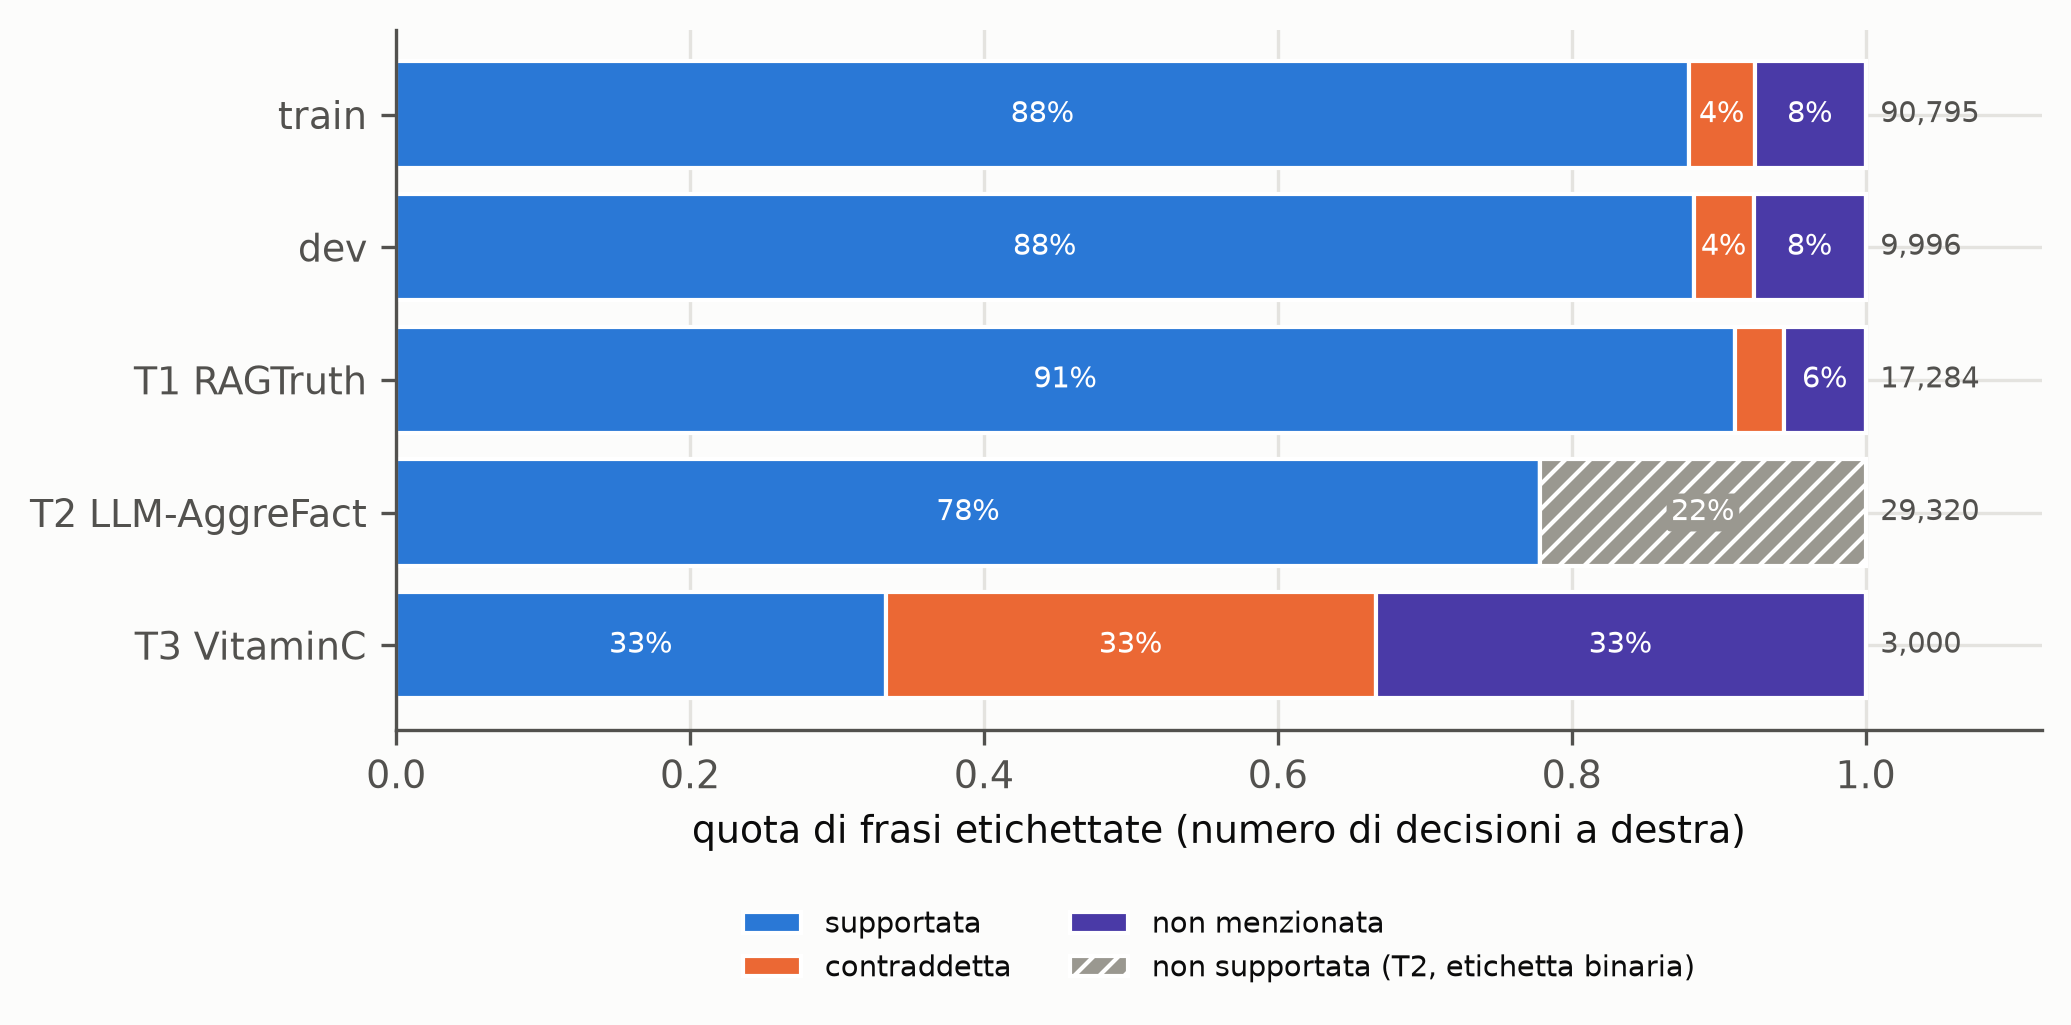
\includegraphics[width=0.9\textwidth]{images/dataset/class_balance_by_split.png}
\caption{Distribuzione delle classi delle frasi etichettate in ciascuna partizione. RAGTruth (addestramento, sviluppo e
T1) è supportato per circa l'88--91\,\%; T3 è campionato a 1{,}000 coppie per classe.}
\label{fig:data-balance}
\end{figure}

\begin{figure}[htbp]
\centering
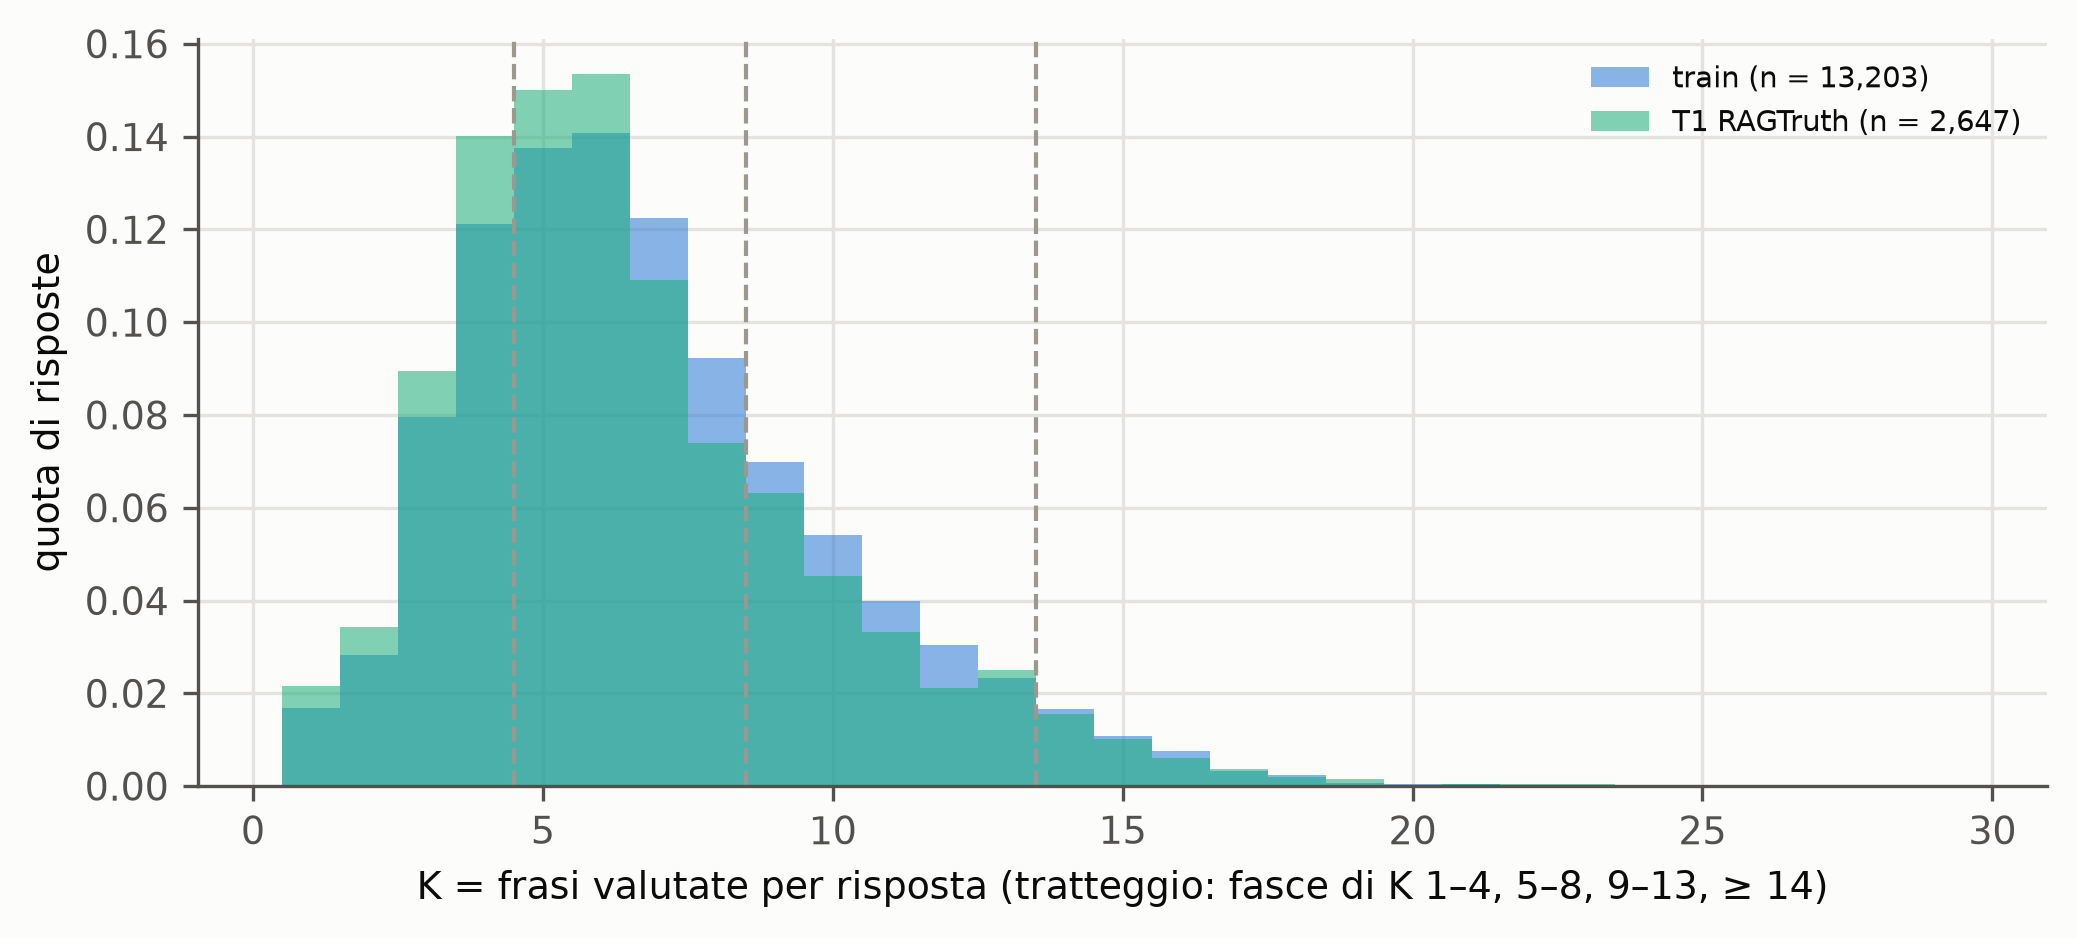
\includegraphics[width=0.9\textwidth]{images/dataset/K_distribution.png}
\caption{Distribuzione di $K$, il numero di frasi valutate per risposta, nell'addestramento e in T1. Le linee
tratteggiate indicano le fasce usate per riportare i risultati in funzione di $K$.}
\label{fig:data-k}
\end{figure}

\section{Affidabilità degli insiemi di test}
\label{sec:data-reliability}

Gli insiemi di test sono stati verificati senza nuove annotazioni, ricorrendo a prove indipendenti dalla costruzione
sopra descritta (Tabella~\ref{tab:data-checks}). Tutte le etichette di test provengono dagli annotatori umani dei
dataset pubblicati. Le due scelte che potrebbero introdurre errori, ossia la segmentazione e la conversione dagli span
alle etichette di frase, sono state confrontate con LLM-AggreFact, i cui autori hanno convertito in modo indipendente le
stesse risposte di test di RAGTruth in affermazioni a livello di frase. Il segmentatore recupera esattamente il
96.3\,\% delle loro affermazioni, e soltanto l'8.5\,\% delle frasi valutate è assente dal loro insieme, per lo più frasi
eliminate dal loro filtro non documentato delle affermazioni ``non degne di verifica''. Sulle 15{,}492 frasi presenti in
entrambi, le etichette binarie concordano nel 98.75\,\% dei casi, e tutti i 193 disaccordi vanno nella stessa
direzione: la regola basata sugli span marca come non supportata una frase che LLM-AggreFact considera supportata.
Infine, un modello di riferimento basato su encoder, valutato su T2 senza modifiche, riproduce il proprio punteggio
pubblicato (74.0 contro 73.5), il che convalida il codice di valutazione.

\begin{table}[htbp]
\centering
\caption{Controlli di affidabilità eseguiti prima che gli insiemi di test venissero congelati.}
\label{tab:data-checks}
\small
\begin{tabularx}{\textwidth}{@{}lXl@{}}
\toprule
Controllo & Criterio & Risultato \\
\midrule
Provenienza delle etichette & ogni etichetta di test proviene da annotatori umani & superato \\
Segmentazione & $\geq$ 90\,\% delle affermazioni di LLM-AggreFact recuperate, $\leq$ 10\,\% delle frasi assenti da esso & 96.3\,\% / 8.5\,\% \\
Derivazione delle etichette & accordo $\geq$ 97\,\% con le etichette binarie di LLM-AggreFact & 98.75\,\% \\
Modello di riferimento & MiniCheck-RoBERTa su T2 entro 1.5 punti dal punteggio pubblicato & 74.0 contro 73.5 \\
Contaminazione & nessuna fonte, documento o coppia (documento, frase) condivisa tra addestramento e test & superato \\
\bottomrule
\end{tabularx}
\end{table}

Questi controlli convalidano il versante binario di T1. La distinzione tra contraddetta e non menzionata si fonda
invece sugli annotatori di RAGTruth, il cui accordo sul tipo di allucinazione non è pubblicato. Inoltre, una recente
ri-annotazione della partizione di test di RAGTruth ha individuato 1.68 volte più risposte allucinate rispetto alle
etichette originali~\cite{yu2026retromorphic}, il che suggerisce che T1 sottostimi le due classi minoritarie. Per questi
motivi i risultati a tre classi su T1 vengono sempre letti insieme a quelli su T3. Dopo questi controlli, e prima che
qualsiasi modello venisse addestrato, i tre file di test sono stati congelati mediante hash crittografici, e il
costruttore del dataset si rifiuta di sovrascriverli con contenuti diversi; ricostruire il dataset a partire dalle
fonti grezze riproduce esattamente i file congelati.

\section{Analisi esplorativa}
\label{sec:data-eda}

Un'analisi esplorativa delle fonti e del dataset costruito ha messo in luce quattro proprietà che determinano il modo
in cui i risultati vanno letti.

\paragraph{Gli errori dipendono dal compito e dal modello.} Le risposte di data-to-text contengono allucinazioni con
una frequenza da due a quattro volte superiore a quella delle risposte negli altri compiti, e le risposte scritte da
Llama-2 e Mistral concentrano la maggior parte delle allucinazioni, mentre quelle di GPT-3.5 e GPT-4 sono quasi sempre
fedeli (Figura~\ref{fig:data-generators}). I risultati vengono quindi riportati per compito, poiché una singola media
rifletterebbe soprattutto il data-to-text.

\begin{figure}[htbp]
\centering
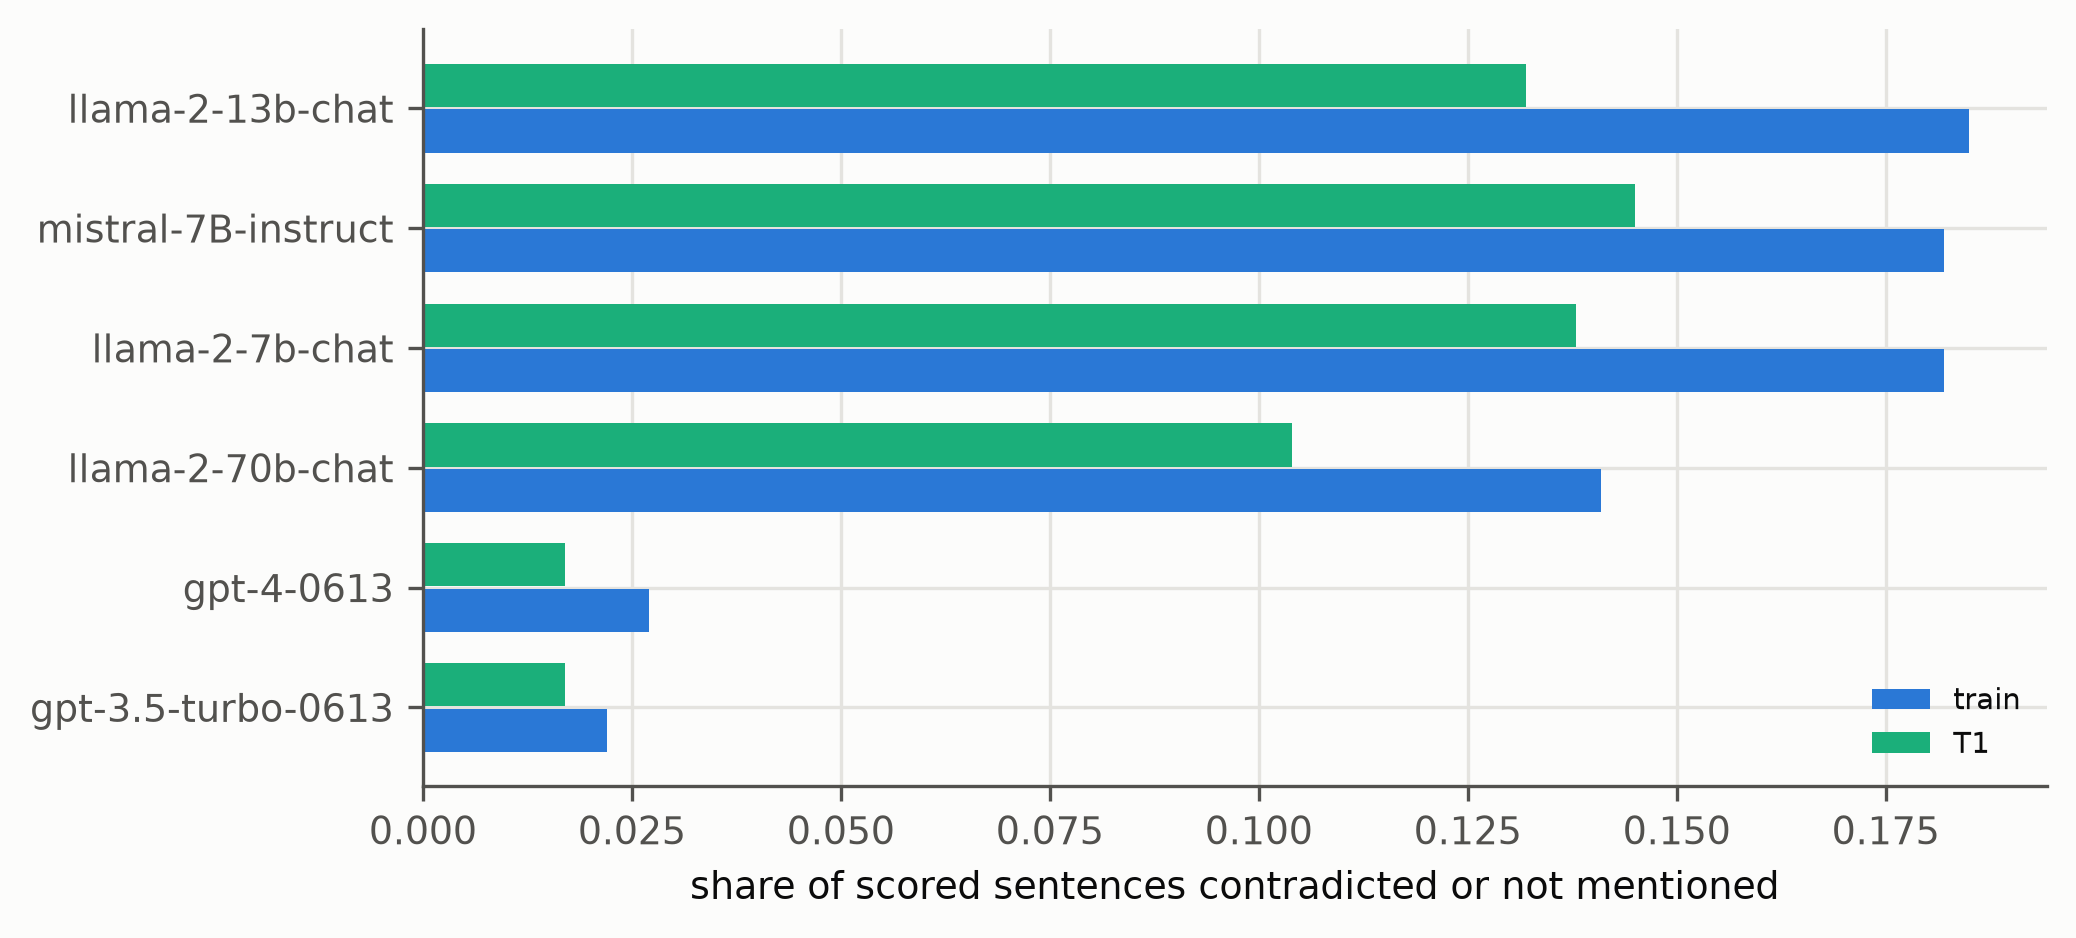
\includegraphics[width=0.9\textwidth]{images/eda/unsupported_by_generator.png}
\caption{Quota di frasi contraddette o non menzionate in base al modello che ha scritto la risposta, nell'addestramento
e in T1.}
\label{fig:data-generators}
\end{figure}

\paragraph{Le risposte di test sono più pulite di quelle di addestramento.} In ogni compito, e per ogni generatore, T1
presenta una quota di frasi contraddette e non menzionate inferiore a quella dell'insieme di addestramento; nella
risposta a domande, per esempio, è contraddetto lo 0.6\,\% delle frasi di T1 contro l'1.6\,\% nell'addestramento. Le
metriche che dipendono dalla frequenza di base, come la precisione o l'F1 sulle classi minoritarie, non sono quindi
confrontabili tra sviluppo e test. Le metriche principali sono l'accuratezza bilanciata, il richiamo macro e l'AUROC,
che non ne dipendono.

\paragraph{Le contraddizioni sono per lo più evidenti.} Circa l'85\,\% delle frasi contraddette di addestramento
proviene da span annotati come conflitti \emph{evidenti}, come numeri o nomi errati, e soltanto 147 da conflitti
\emph{sottili}. La classe contraddetta è dunque composta per lo più da contraddizioni palesi, e le contraddizioni sottili
non possono essere valutate separatamente.

\paragraph{Gli indizi superficiali esistono e definiscono i modelli di riferimento.} Due semplici indizi predicono le
etichette senza verificare la frase rispetto al documento. Il primo è la sovrapposizione lessicale. La quota di parole
di contenuto di una frase che compaiono anche nel documento è più alta per le frasi supportate che per quelle
contraddette e non menzionate, in tutti e tre gli insiemi di test (Figura~\ref{fig:data-overlap}). Da sola, essa separa
le frasi supportate da quelle non supportate con un AUROC di 0.74 su T1 e di 0.70 su T3. Il secondo indizio è la
formulazione della frase. Un classificatore basato sulla sola frase raggiunge un'accuratezza bilanciata a tre classi di
0.66 sul data-to-text, poiché alcuni dettagli, come il numero di recensioni o la disponibilità di Wi-Fi o di parcheggio
con valet, vengono spesso inventati nelle descrizioni di Yelp. Nella risposta a domande e nel riassunto lo stesso
classificatore resta al livello del caso (0.36 e 0.35), e così anche su T3 (0.33), dove il disegno contrastivo elimina
l'indizio. Un verificatore è utile solo nella misura in cui supera questi indizi, e per questo entrambi vengono
riportati come modelli di riferimento, per compito.

\begin{figure}[htbp]
\centering
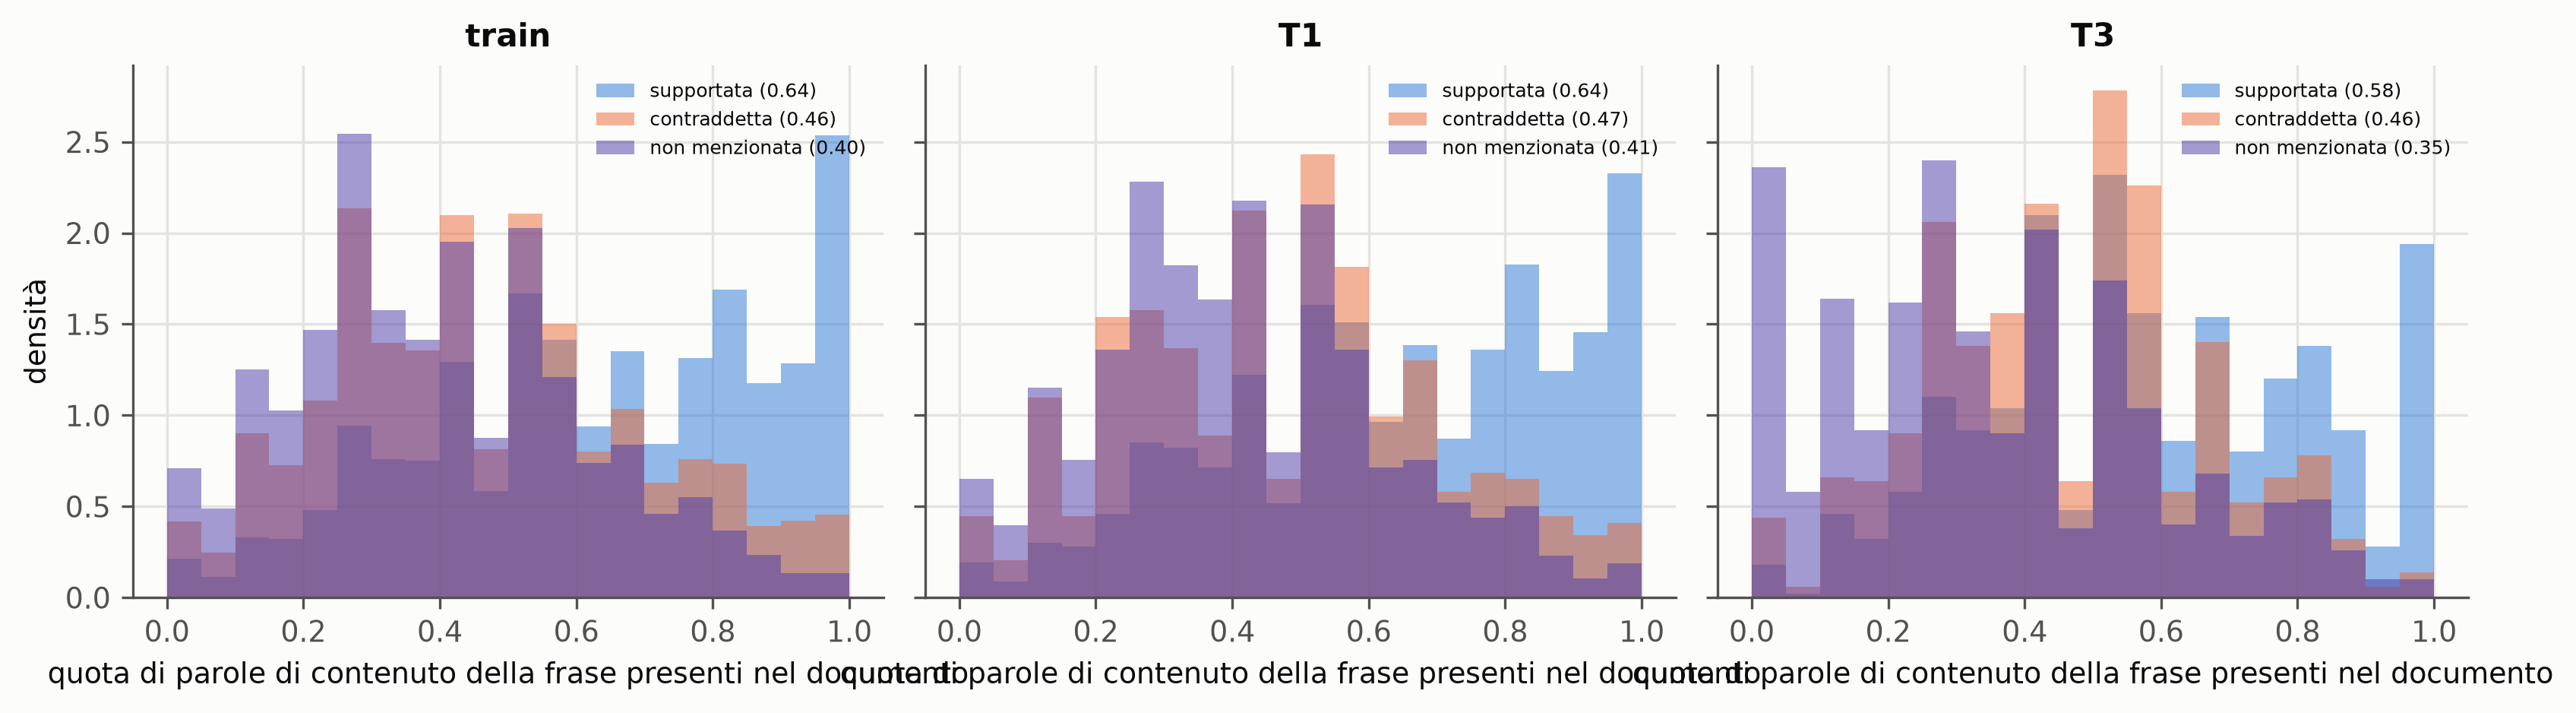
\includegraphics[width=\textwidth]{images/eda/overlap_by_class.png}
\caption{Sovrapposizione lessicale tra una frase e il suo documento, per classe, nell'addestramento, in T1 e in T3
(media tra parentesi).}
\label{fig:data-overlap}
\end{figure}

Infine, le frasi non supportate non si concentrano alla fine della risposta. La prima frase è raramente non supportata,
la quota raggiunge il massimo nelle posizioni dalla terza alla quinta e resta tra l'8 e l'11\,\% nelle posizioni
successive (Figura~\ref{fig:data-position}). Anche le risposte lunghe contengono errori verso la fine, e l'accuratezza
per valori elevati di $K$ è quindi rilevante.

\begin{figure}[htbp]
\centering
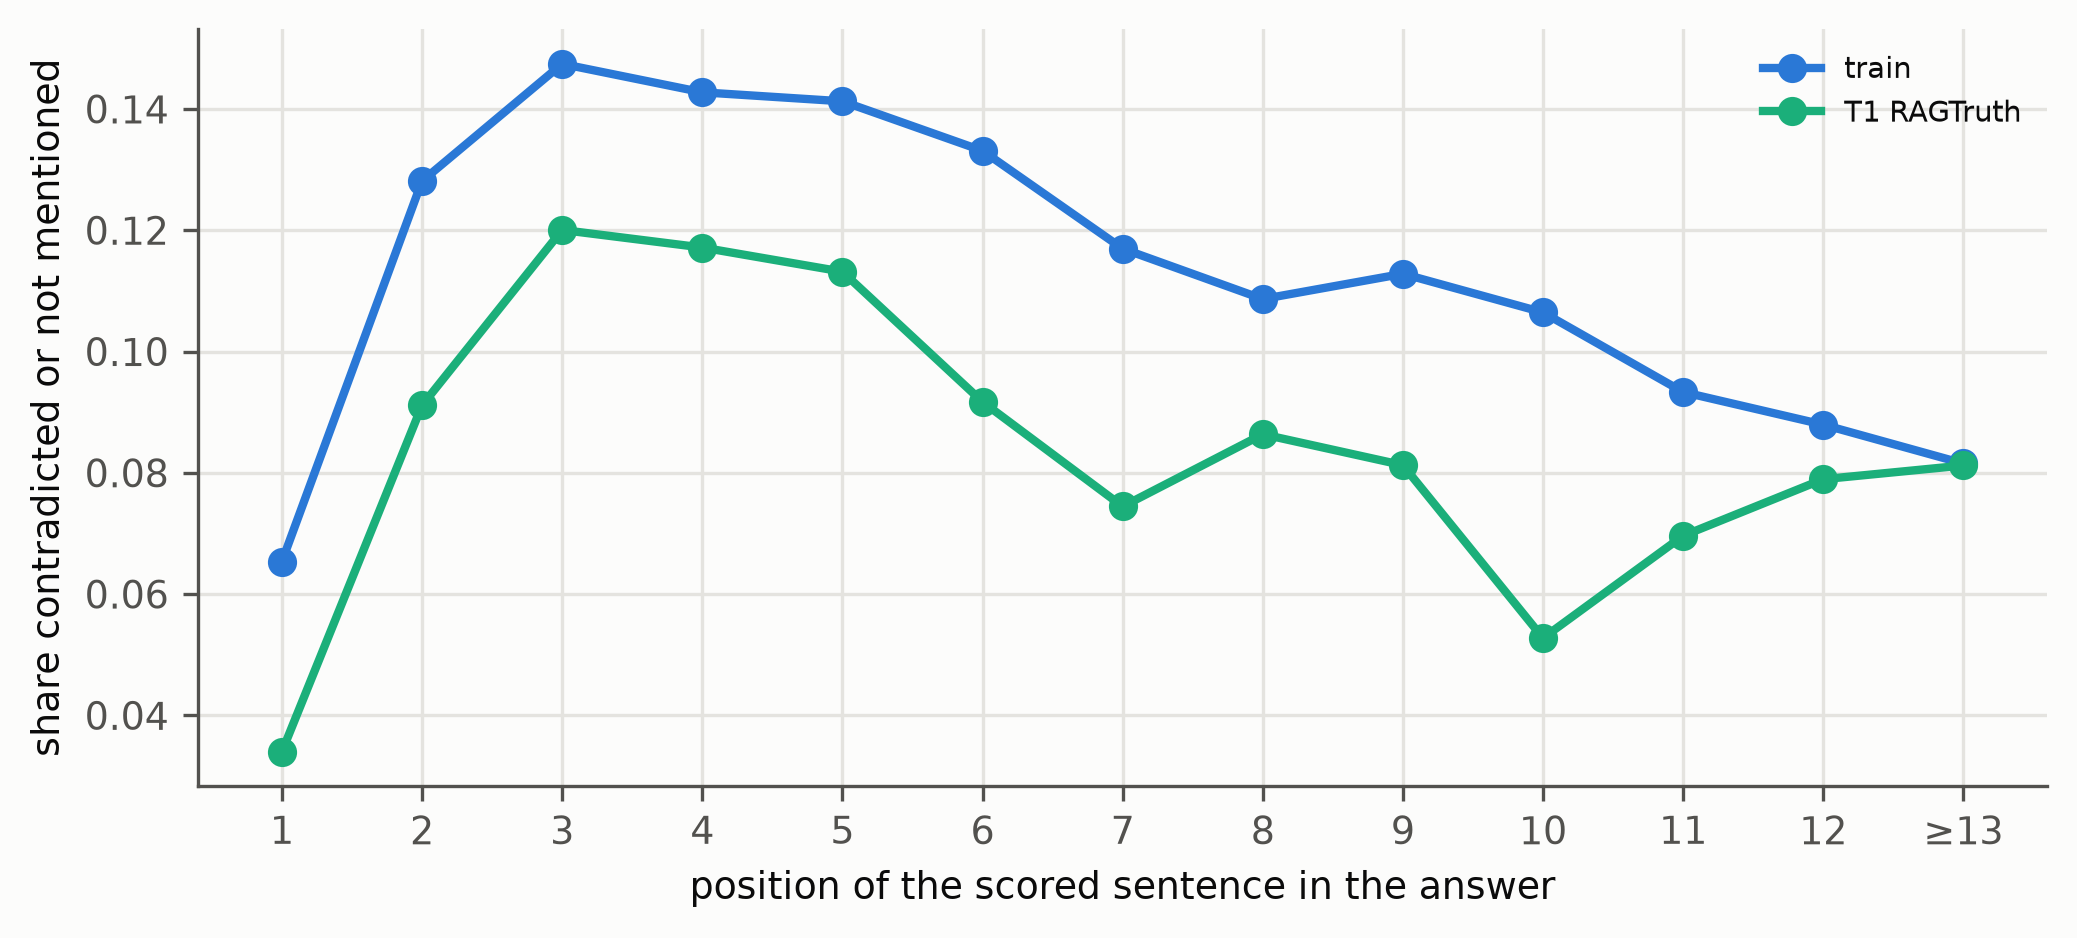
\includegraphics[width=0.9\textwidth]{images/dataset/unsupported_by_position.png}
\caption{Quota di frasi contraddette o non menzionate in base alla posizione nella risposta.}
\label{fig:data-position}
\end{figure}

\section{Controllo della contaminazione (leakage)}
\label{sec:data-leakage}

Le partizioni sono definite per fonte, mai per frase, e un controllo automatico viene eseguito a ogni costruzione. Il
controllo fallisce se una fonte, un documento o una coppia (documento, frase) dell'insieme di addestramento o di
sviluppo compare in uno qualsiasi degli insiemi di test, oppure se gli insiemi di sviluppo e di addestramento
condividono una fonte. Il controllo risulta superato. Esso segnala inoltre le stringhe di frase che ricorrono sia
nell'addestramento sia nel test con documenti diversi: si tratta di 788 frasi modello, come ``The business has a rating
of 4.0 stars.'', attese nel data-to-text e che non rivelano alcuna etichetta di test. Non è possibile verificare se i
dataset pubblici qui impiegati facessero parte dei dati di pre-addestramento di Qwen2.5, e questo resta un limite
condiviso dalla maggior parte dei lavori basati su benchmark pubblici.
